% This is the chapter 'Action Potential' to the "Hodgkin-Huxley  neuron model V2.0 book"
% Last edited 2026.06.24

\chapter{Action Potential\label{ch:ActionPotential}}


As discussed, a smaller number of ion channels is distributed over the surface of the membrane, and the overwhelming majority of ion channels is concentrated in the \gls{AIS}.


\section{The physical process\label{sec:AP-PhysicalProcess}}

In the resting state, we have a condenser that has some low-conductance resistors (the resting ion channels) and a very low intensity (nearly constant) distributed current flows, under the effect of a slightly varying (nearly constant) membrane voltage. Due to the membrane potential, a current through the always-open channels flows on the dendritic surface
and the resting channels' conductivity represents a drain with 
sufficient transmission. The resting current practically does not 
reach the \gls{AIS}: the ion channels along the current's path
practically "shunt" the current.
This is a static state that classical neuroscience assumes: some static current in and some static (leakage) current out; no significant gradient.
\textit{In this state}, an almost correct model is a condenser with a
\textit{parallelly} switched resistor; an integrator-type  $RC$ circuit, see Table~\ref{tab:Electric_RCOscillator_Circuits}
(although when approaching the threshold voltage, the \gls{AIS} plays some role. The smaller gradient changes, such as subthreshold excitations, produce "mini-\gls{AP} waves"~\cite{NeuralEnergyConsumption:2017}, providing direct experimental proof that in this state the parallel $RC$ circuit is not correct).
Some perturbations must be counterbalanced, but their
amount does not exceed a predefined threshold.

In the transient (perturbed) state, the process variable
(the membrane's potential) exceeds the threshold. That event acts
as a fast trigger signal. The amount of charged particles (and so:
the membrane's voltage) suddenly increases, the created gradient
drives a current.
When $Na^+$ ions rush into the intracellular layer, they roughly increase the overall concentration and the potential in that thin layer.
All nearby ions feel a driving force. The targeted membrane potential is set electrically,
and the driving gradients may behave in unexpectedly during the transient period.
The actual voltage gradient may temporarily reverse the direction of the chemical gradients.

Our results align with the observation (see caption of 11.22 in~\cite{MolecularBiology:2002}), that \textit{the significant processes
	occur in a thin layer of the electrolyte proximal to the membrane surface}.
The amount of unbalanced ions is in the range of $10^7$,
and so is the amount of rush-in ions. In addition, those 
ions on the high-concentration side rush into the 
low-concentration side and cause a significant change in the 
membrane potential (and concentration). Their absolute amount is small compared to the total number of ions in the cell,
but it is significant compared to the number of unbalanced ions in that layer.
However, the layer itself can also be modeled
as having just a few ions under their mutual repulsion on the surface
or in a few atomic layers on top of each other, depending on the concentration.



Suppose that at the beginning of an \gls{AP} a large amount of $Na^+$ ions are transferred from the extracellular to the intracellular side. In that case,  the $K^+/Na^+$ concentrations change from $145/15$ to $45/115$ and the 
corresponding thermodynamic voltage contribution changes from $+61\ [mV]$ to $-25\ [mV]$ (i.e., altogether a $86\ [mV]$ sudden increase in membrane potential). For the $Na^+$ ions, the resultant potential changes from $+4\ [mV]$ to $-83\ [mV]$. That means when the \gls{AP} begins, the "Na-K pump" stops (if the resulting potential provides the driving force for the exchange pump). The only way for the neuron to remove the excess  $Na^+$ ions is to generate a current toward the \gls{AIS} (where the other end of the ion channels remained at the extracellular potential), until the $Na^+$-specific driving force disappears. The $K^+$-specific driving force, changes from $-90\ [mV]$ to  $-176\ [mV]$, i.e., the $K^+$
intake gets more intensive, misleading researchers into believing that it causes
the observed hyperpolarization. However, as  Fig.~3 in~\cite{NeuralEnergyConsumption:2017} demonstrates, it occurs instantly, not with a delay; furthermore, the "leakage current" and the stimulus current are negligible. The low extracellular $K^+$ concentration plus the 
low number of channels in the membrane's wall
do not enable a significant increase in the intracellular $K^+$. 
(Given that complex changes occur, including changes in the electrical potential that also change the concentrations, different waves start; the statement is not strictly valid.)

%	Fig.~\ref{fig:AP-K_to_Na} attempts to give a feeling how the effective driving force exerted on $Na^+$ and $K^+$ changes when generating an \gls{AP}. The voltage shown on the vertical scale is the resulting driving force at a given time (Of course, the voltage depends on the time and the location; for an exact time course a detailed multi-physics simulation is needed). The ions feel an outward driving force if
%	the resulting local thermodynamic plus electrical potential is positive
%	and an inward driving force otherwise. As the figure shows, the $Na^+$ ions feel an outward driving force when the membrane's voltage is
%	above the threshold, while the $K^+$ ions feel at the same time mostly 
%	inward driving force. The ratio of the driving forces 
%	(and consequently the amount of the transported mass) changes continuously during generating the \gls{AP} 
%
%
%\begin{figure}
%	\includegraphics[,trim={.5cm -0.cm 0cm 0cm},
%	scale=1.6]{AP_K_to_Na.pdf}
%	\caption{A rough illustration of how the effective driving force
	%		changes during generating an \gls{AP}. 		
	%		\label{fig:AP-K_to_Na} 	}
%\end{figure}
%
As the current flows, the thermodynamic force decreases, and at some point the resultant force changes its sign; so does the current direction. This is seen as the "condenser current" (and mis-identified as an intense $K^+$ current). The ions move slowly, and due to the enormous electrostatic repulsion, their "electrostatic fluid" must be continuous. A special "damped wave" is formed (with all secondary mechanical, optical, etc. effects) and the condenser current reverses. Electricity interprets the phenomenon as "capacitive current" in the equivalent circuit, and thermodynamics interprets it as 
changed chemical concentration (or the negative amplitude of the damped elastic oscillation). Our discussion adds that electrical repulsion generates a pressure wave, or shock wave, within the neuron's closed volume.


\begin{figure}
	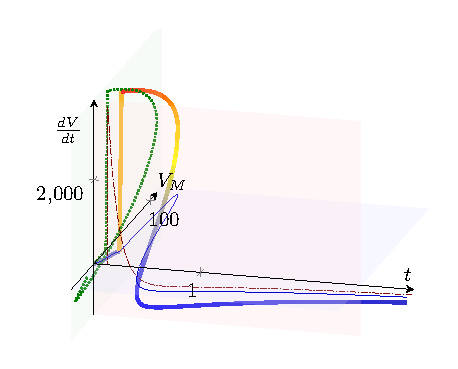
\includegraphics[,trim={.5cm -0.cm 0cm 0cm},
	scale=1.5]{fig/dVdt_vs_V_3d}
	\caption{A summary of producing neuronal \gls{AP} as a 3-D figure. The thick, solid 3-D line shows how the color-coded voltage gradient drives the membrane potential over time.
		The three dashed diagram lines are the projections of the 
		spatial curve to the boundary planes of the cube. The physiology delivers them as 2-D plots; the figure explains how those parameters are interrelated. 
		The red line shows the voltage gradient
		produced by the rush-in of the $Na^+$ ions, see also 
		the middle inset in Fig.~\ref{fig:PhysicalProcessesMembrane}.
		The blue diagram line shows the \gls{AP}, see also 
		the bottom inset in Fig.~\ref{fig:PhysicalProcessesMembrane}.
		The interdependence of the gradient and the voltage is called a phase plot; see, for example~\cite{BeanActionPotential:2007}.		
		\label{fig:SummaryPicture} 	}
\end{figure}

The neuronal \gls{AP} generation can be entirely described  
by the 3-D line in 
Fig.~\ref{fig:SummaryPicture}. The three dashed diagram lines are drawn in 
three perpendicular planes; see the figure's caption and the discussion below for the details.


\section{The oscillator model\label{sec:OscillatorModel}}

Despite the early warning that '\textit{it was not possible to separate the change into
	resistance and capacity components}' \cite{COLE_CURTIS_IMPEDANCE:1939},
a commonly accepted truism was that neurons, in some sense, behave
as electrical oscillators.
\gls{HH} introduced the idea explicitly that the electrically equivalent circuit
of a neuron is an $RC$ oscillator.
We must also add the invention from about three decades later: "Neurons ensure the directional propagation of signals throughout the nervous system.
The functional asymmetry of neurons is supported by cellular compartmentation: the cell body and dendrites (somatodendritic compartment) receive synaptic inputs,
and the axon propagates the action potentials that trigger synaptic release toward target cells.
\textit{Between the cell body and the axon sits a unique compartment called the axon initial segment}.
The \gls{AIS} was first described 50 years ago [i.e., nearly two decades after \gls{HH} published their study], and its molecular composition
and organization have been progressively elucidated during the following decades. \dots.
Recent years have also brought crucial insights into the functions of the \gls{AIS}:
how \textit{ion channels at its surface generate and shape the action potential}."~\cite{AIS_Updated_Viewpoint:2018}
We provide the physics and mathematics of how \gls{AIS} shapes
the action potential (or more precisely, we show what an important role it plays in forming \gls{AP}).

Inventing \gls{AIS} changed the viewpoint of neuroscience~\cite{AIS_Updated_Viewpoint:2018}, a half century later, after setting up the commonly accepted model by \gls{HH}.
"The \gls{AIS} is located at the proximal axon and is the site of action potential initiation. This
reflects the high density of ion channels found at the \gls{AIS}.
... The summation of
synaptic inputs gives rise to action potentials at the
\gls{AIS}, a 20--60 $\mu m$ long domain
located at the proximal axon/soma interface that has
a high density of voltage-gated ion channels."	
As discussed in \cite{AISStructureReview:2018}, see also their Figure 1, 
the structure of the \gls{AIS}
is known to the most minor details.
As the illuminating investigations in 2008
\cite{ActionPotentialGenerationNatrium:2008}
revealed, the 
\gls{AIS}
has very dense ion channels. That is, from an electrical point
of view, those parallelized channels can be abstracted as a  \textit{discrete  conductance}
(or resistance) between the membrane and the axon.
The membrane itself can be abstracted as a \textit{distributed condenser} with no resistance.
This model is in contrast with the viewpoint of biophysics, that the membrane plus \gls{AIS}
is considered a distributed element, where the capacitor and condenser cannot be separated. The current model is the result of projecting the physical processes in the resting state to the transient state.
Notice the important point:
"Neurons are also anatomically polarized, as they can be
subdivided into a somatodendritic input domain and an axonal output domain"~\cite{AIS_NeuronalPolarity:2010};
providing direct evidence that (unlike in 
\gls{HH}'s
model)\textit{ the input and output currents (and voltage time derivatives) are independent}.

\begin{table}
	\caption{\href{href="https://www.electronics-tutorials.ws/rc/rc-integrator.html} {RC circuit types}\label{tab:Electric_RCOscillator_Circuits}}
	\centering
	\begin{tabular}{cc}
		\hline
		\hline
		The RC Integrator
		\label{RCIntegratorCircuit}                                                                                                                                   & The RC differentiator                                                                                                                                  \label{RCDifferentiatorCircuit}                                                                                                                                  \\
		\hline
		$
		V_{out}^{Integrator}=\frac{1}{RC}\int_0^t V_{in}{dt}\label{eq:RC_Integrator}
		$
		& $V_{out}^{Differentiator}=RC\frac{dV_{in}}{dt} $ \\
		\hline
		Low Pass Filter&\textbf{High Pass Filter}\\
		\hline
		Resting state&\textbf{Transient state}\\
		\hline
		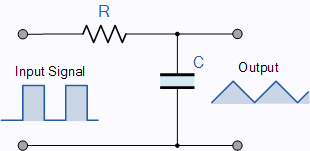
\includegraphics[width=.4\textwidth]{fig/rc-rc12Integrator.jpg} & 
		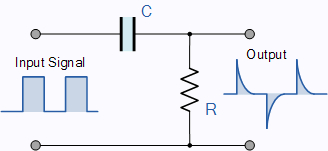
\includegraphics[width=.42\textwidth]{fig/rc-rc13Differentiator.jpg}\\
		\hline
		(Mostly) resting state& (Mostly) transient state\\
		\hline
		Ion channels in the membrane&
		Ion channels in the AIS\\
		\hline
	\end{tabular}
\end{table}


In our model, the 
\gls{AIS} gets part of the membrane,
and this leads to crucial changes. (BTW, the name is slightly misleading:
the \gls{AIS} is part of the neuronal oscillator, and it forwards a traveling
potential wave to the axon instead of belonging to it.)
'Although by definition a neuron must have an
axon to assemble an \gls{AIS}, the relationship between \gls{AIS}
assembly and axon specification in vivo has not been
determined yet'~\cite{AIS_NeuronalPolarity:2010}.
Anyhow, a neuron can be abstracted (in the disciplinary view of electricity) as comprising a resistor-like and a capacitor-like component. However, in the resting and the transient states, they are combined in different ways.




In the resting state, we can model neurons as a \textit{parallel} $RC$ circuit (see the "integrator" in Table~\ref{tab:Electric_RCOscillator_Circuits}), where "random" currents flow in and out. Practically,
the output voltage is constant (the resting potential): the
ion channels and pumps are distributed over the membrane's surface,
and due to the low speed of currents, at low local voltage gradients,
the \gls{AIS} is not involved. Only the synaptic inputs cause a
measurable gradient on the \gls{AIS}. In this native state, there is no gradient; in this sense, it is similar to the case of clamped operation, where the gradient is (apparently) suppressed by the feedback.
\gls{HH} did not see any structural elements on the membrane,
so logically, they modeled it as a distributed resistor and capacitor,
which really has resemblance with a \textit{parallel $RC$ oscillator.}
However, they made a wrong choice of the circuit type, and their choice (likely due to inertia)
was repeated in good textbooks such as  (\cite{ JohnstonWuNeurophysiology:1995}
Figure 3.1 or \cite{KochBiophysics:1999} Figure 1.1), and
it is a commonly accepted fallacy even today~\cite{NeuralDynamicsGertsner:2014}.


In the transient state,  the 
high-transmission ion channels in the \gls{AIS} (high conductance $R$) replace the low-transmission ion channels (low conductance $R$) in the membrane's wall, and the rush-in current flows out entirely on the \gls{AIS}
(for the model, in this state, we omit the low-transmission ion drain).  
Those two elements form a \textit{serial} $RC$ circuit (see the "differentiator" in Table~\ref{tab:Electric_RCOscillator_Circuits}) that acts as a damped oscillator and produces a current pulse, known as \gls{AP}. Neuroscience mistakenly claims it is a parallel $RC$ circuit; that statement is valid only in the resting state.
However, the number and intensity of the 'resting' ion channels in the membrane's wall are insignificant for producing \gls{AP}, so  we use the approximation that only the 'transient ion channels' in the \gls{AIS} 
are active when generating an \gls{AP}.   
%In this action, the gated ion channels in the membrane's wall produce an instant pulse (see Figure~\ref{fig:PhysicalProcessesMembrane} middle inset) that appears as a peaked current (see Figure~\ref{fig:PhysicalProcessesMembrane} bottom inset) due to the slowness of the charge carriers and that the ion channels for the rush-in current are distributed on the membrane's surface. The output current flows as long as the offset potential persists.


In the electrical view, the process can be modeled as follows: a sudden voltage gradient  (see Figure~\ref{fig:PhysicalProcessesMembrane} middle inset) appears on the membrane (as a discrete capacitor), and a current flows out (see Figure~\ref{fig:PhysicalProcessesMembrane} bottom inset) through the serially connected ion channel array (as a discrete resistor). The neuron forms a simple \textit{serially }(\textit{not parallelly}, as assumed by Hodgkin and Huxley~\cite{HodgkinHuxley:1952} and mistakenly claimed by neurophysiology) connected $RC$ oscillator.
For the physical and mathematical description, see section~\ref{sec:MathematicsAP}, furthermore, ~section~4 in~\cite{VeghTechnomorphBiology:2025}; for its algorithmic specifics~\cite{VeghNeuronAlgorithms:2025}, for further details~\cite{VeghDANCES:2026}.
Notice that the difference between the rush-in and the resultant gradients
emphasizes the role of the finite resources: without the \gls{AIS},
no turn-back of the resultant gradient would occur.


\begin{figure}[]
	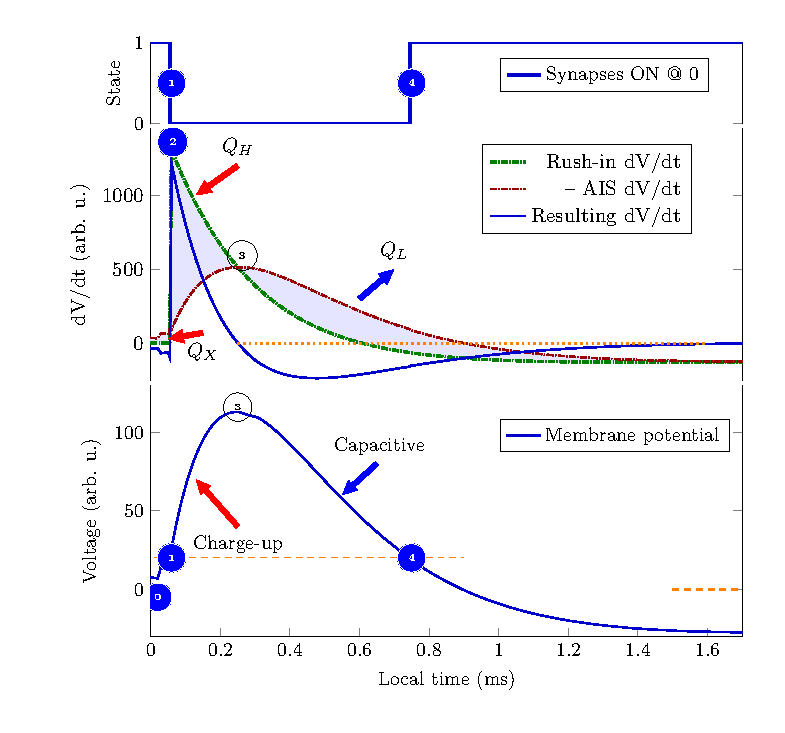
\includegraphics[scale=1]{fig/AP_Artificial_test}
	
	\caption{The physical processes describing the membrane's operation\label{fig:PhysicalProcessesMembrane}. The rush-in $Na^+$ ions instantly increase the membrane's charge, and the membrane's capacity discharges (producing an exponentially decaying voltage derivative). The ions are created at different positions on the membrane, so they take different times to reach the \gls{AIS}, where the current produces a peak in the voltage derivative. The resulting voltage derivative, the sum of the two derivatives (the \gls{AIS} current is outward), drives the oscillator. Its integration produces the membrane potential. When the membrane potential crosses the threshold, it switches the synaptic currents on or off.}
	
\end{figure}

The fundamental difference between the parallel and serial $RC$ circuits is that \textit{the parallel circuit cannot produce output voltage with opposite sign}. 
As discussed, the capacitive current, which by definition changes its direction and so 
generates an opposite voltage on the resistor represented by the \gls{AIS}, perfectly describes the so-called "hyperpolarization". It is not the effect of a $K^+$ current: the resting ion channels do not have sufficient conductance.  
Not knowing about the \gls{AIS} leads to assuming that the resting ion channels work also as transient channels (in other words, assuming a parallel $RC$ circuit instead of the serial one, furthermore, that
the output current flows through the membrane instead of the axon). Some $K^+$ current certainly exists; for the magnitude of currents during \gls{AP}, see~\cite{NeuralEnergyConsumption:2017}.


The shape of the output waveform depends on the ratio of the pulse width to the $RC$ time constant. When $RC$ is much larger than the pulse width, the output waveform resembles the input signal, even with a square wave input. (In the case of the neuronal oscillator, the shape of the front side of the spike is similar to the one derived for the rush-in current, while the back side is very prolonged.)


\section{Mathematics of the ActionPotential\label{sec:MathematicsAP}}

Although the implementation of a neuronal circuit works with ionic
currents and has a charge transmission mechanism drastically different
from the one based on free electrons used in metals, the operation
can align (to some measure) with the instant currents of physical
electronics (as we suggest, the effect of the slow current and finite
size can be reasonably imitated with current generators generating
a special current shape). The input currents in a biological circuit
are a large rush-in current through the membrane in an extremely short
time, and much smaller gated synaptic currents arriving at different
times through the synapses. Those currents generate voltage gradients,
and those gradients direct the operation of the $RC$ oscillator
(Notice that due to the multi-physical effects, the parameters $R$ and $C$ may change in the function of time and the actual voltage).
As it is well known from the theory of electrical circuits, the output
voltage measured on the output resistor is as follows:

\begin{equation}
	V_{out}^{Differentiator}=RC\frac{dV_{in}}{dt}\label{eq:RC_Circuit_Output}
\end{equation}

\noindent where the input voltage is as follows:

\begin{equation}
	\frac{d}{dt}V_{in}=\sum\frac{d}{dt}V_{IN}^{Component}-\frac{d}{dt}V_{OUT}^{AIS}\label{eq:RC_Circuit_Input}
\end{equation}

\noindent that is, the (temporally gated) sum of the input gradient
that the currents generate, plus the gradient of the output current
through the \gls{AIS}~\cite{AISStructureReview:2018,AIS_Updated_Viewpoint:2018}.
The latter term can be described as follows (see the discussion around also Eq.(\ref{eq:PID}):
\begin{equation}
	\frac{d}{dt}V_{OUT}^{AIS}={\frac{1}{C}}\frac{V_{internal}-V_{external}}{R_{AIS}}\label{eq:AIS_Voltage}
\end{equation}

The input currents are slow (we typically imitate them using a current generator with a special form).
In the simplest case, the resulting voltage derivative comprises only
the rush-in contribution %described by Equation~(\ref{eq:PSPderivative})
and the \gls{AIS} contribution described by Equation~(\ref{eq:AIS_Voltage}).
The gating implements a dynamically changing temporal window and dynamically
changing synaptic weights. The appearance of the first arriving synaptic
gradient starts the ``Computing'' stage. The rush-in gradient starts
the ``Delivering'' stage~\cite{VeghNeuronAlgorithms:2025}. The charge collected in that temporal window is as follows: 
\begin{equation}
	Q(t)=\int_{t_{0,i}}^{{t_{thr}}}dt\underbrace{\sum_{i}}_{{t_{0,i}\le t\le t_{thr}}}I_{syn,i}(t)
\end{equation}

The total charge is integrated in a mathematically entirely unusual
way: this is \textit{NOT} a simple "integrate and fire": the collected charge defines the upper bound of the integration time. Through adjusting the integration time window, the neuron selects which
one(s) out of its upstream neurons can contribute to the result; the
individual contributions are the result of a bargain between the sender and the
receiver. The upstream neuron decides when the time window begins, but the neuron decides when a contributing current terminates. \emph{The beginning
	of the time window is set by the arrival of a spike from one of the
	upstream neurons, and it is closed by the neuron when the charge integration
	results in a voltage exceeding the threshold.}
The speculations~\cite{MechanicalPropertiesNerves:2025} about the spatial length of the spike are correct, but its "payload length" is defined by the receiving neuron. The computation (a
weighted summation) is performed on the fly, excluding the obsolete
operands (the
idea of \gls{AIMC}~\cite{AnalogInMemoryComputing:2024}
almost precisely reproduces the charge summation except for timing). The
only operation that a neuron can perform is that unique integration.
Its result is the reciprocal of the weighted sum, and it is represented
by the time when a spike is sent out (\emph{when} that charge on the
membrane's fixed capacity leads to reaching the threshold). Notice
that the time is defined on the neuron's local time scale and is interpreted
similarly by the downstream neurons: the data transmission time matters.

